\addtocounter{section}{-1}
\section{Chapter Prerequisites}
\prereqIntro

\subsection*{Functions}

A \textbf{function} $f$ is a rule that assigns each element $x$ from a set (called the domain) to exactly one element, called $f(x)$, in another set. Unless we say otherwise, the \textbf{domain} is the set of all real numbers for which the rule makes sense and defines a real number. All possible values of $f(x)$ are called the \textbf{range} of $f$. We use four ways to represent a function.\\
\begin{minipage}{.5\linewidth}
\begin{itemize}
\item By a graph
\item By an explicit formula
\end{itemize}
\end{minipage}%
\begin{minipage}{.5\linewidth}
\begin{itemize}
\item By a table of values
\item By a verbal description
\end{itemize}
\end{minipage}

Throughout the book we will use several representations of any given function to help give us a better understanding of the problem. The graphs in \autoref{prereq_basic_graphs} contain most of the base functions we can use to build other functions using transformations.

%\ifthenelse{\boolean{latexml}\OR\isodd{\thepage}}{%
%% do nothing
%}{%
%\hspace{-70pt}%
%}%
\begin{lxfigure}
\begin{center}
\begin{tabular}{c c c}
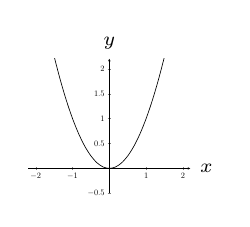
\begin{tikzpicture}[scale = .3]
\begin{axis}[axis y line=middle, axis x line=middle, xmin=-2.2, xmax=2.2, ymin=-.5, ymax=2.2,name=myplot]
\addplot[{\colorone}, domain=-2:2, thick, smooth]{x*x};
\end{axis}
\node [right] at (myplot.right of origin) {\scriptsize $x$};
\node [above] at (myplot.above origin) {\scriptsize $y$};
\end{tikzpicture}
&
\begin{tikzpicture}[scale = .3]
\begin{axis}[axis y line=middle, axis x line=middle, xmin=-.5, xmax=3.2, ymin=-.5, ymax=2.2,name=myplot, ytick={0, 1,2}, xtick={0,1,2,3}]
\addplot[{\colorone}, domain=-0:3, thick, smooth,samples=100]{sqrt x};
\end{axis}
\node [right] at (myplot.right of origin) {\scriptsize $x$};
\node [above] at (myplot.above origin) {\scriptsize $y$};
\end{tikzpicture}
&
\begin{tikzpicture}[scale = .3]
\begin{axis}[axis y line=middle, axis x line=middle, xmin=-2.2, xmax=2.2, ymin=-.5, ymax=2.2,name=myplot, ytick={0, 1,2}]
\addplot[{\colorone}, domain=-2:2, thick, smooth]{abs x};
\end{axis}
\node [right] at (myplot.right of origin) {\scriptsize $x$};
\node [above] at (myplot.above origin) {\scriptsize $y$};
\end{tikzpicture} \\
$y=x^2$ & $y=\sqrt x$& $y=\abs{x}$
\\
\begin{tikzpicture}[scale = .3]
\begin{axis}[axis y line=middle, axis x line=middle, xmin=-2.2, xmax=2.2, ymin=-2.2, ymax=2.2,name=myplot]
\addplot[{\colorone}, domain=-2:2, thick, smooth]{x*x*x};
\end{axis}
\node [right] at (myplot.right of origin) {\scriptsize $x$};
\node [above] at (myplot.above origin) {\scriptsize $y$};
\end{tikzpicture}
&
\begin{tikzpicture}[scale = .3]
\begin{axis}[axis y line=middle, axis x line=middle, xmin=-2.2, xmax=2.2, ymin=-.5, ymax=3.2,name=myplot, ytick={0, 1,2,3}]
\addplot[{\colorone}, domain=-2:2, thick, smooth]{e^x};
\end{axis}
\node [right] at (myplot.right of origin) {\scriptsize $x$};
\node [above] at (myplot.above origin) {\scriptsize $y$};
\end{tikzpicture}
&
\begin{tikzpicture}[scale = .3]
\begin{axis}[axis y line=middle, axis x line=middle, xmin=-.5, xmax=3.2, ymin=-2.2, ymax=2.2,name=myplot, ytick={-2,-1,0, 1,2},xtick={0,1,2,3}]
\addplot[{\colorone}, domain=.01:3, thick, smooth]{ln x};
\end{axis}
\node [right] at (myplot.right of origin) {\scriptsize $x$};
\node [above] at (myplot.above origin) {\scriptsize $y$};
\end{tikzpicture} \\
$y=x^3$ & $y=e^x$& $y=\ln x$
\\
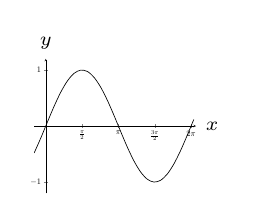
\begin{tikzpicture}[scale = .3]
\begin{axis}[axis y line=middle, axis x line=middle, xmin=-.5, xmax=6.5, ymin=-1.2, ymax=1.2,name=myplot, ytick={-1,0,1}, xtick={-6.28318, -4.7123889, -3.14159, -1.5708, 1.5708, 3.14159, 4.7123889, 6.28318}, xticklabels={-$2\pi$, $-\frac{3\pi}{2}$,$-\pi$, $-\frac{\pi}{2}$, $\frac{\pi}{2}$,$\pi$, $\frac{3\pi}{2}$, $2\pi$}]
\addplot[{\colorone}, domain=-.5:6.4, thick, smooth]{sin deg(x)};
\end{axis}
\node [right] at (myplot.right of origin) {\scriptsize $x$};
\node [above] at (myplot.above origin) {\scriptsize $y$};
\end{tikzpicture}
&
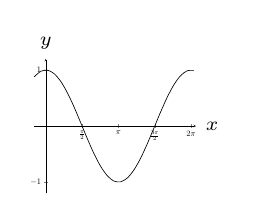
\begin{tikzpicture}[scale = .3]
\begin{axis}[axis y line=middle, axis x line=middle, xmin=-.5, xmax=6.5, ymin=-1.2, ymax=1.2,name=myplot, ytick={-1,0,1}, xtick={-6.28318, -4.7123889, -3.14159, -1.5708, 1.5708, 3.14159, 4.7123889, 6.28318}, xticklabels={-$2\pi$, $-\frac{3\pi}{2}$,$-\pi$, $-\frac{\pi}{2}$, $\frac{\pi}{2}$,$\pi$, $\frac{3\pi}{2}$, $2\pi$}]
\addplot[{\colorone}, domain=-.5:6.4, thick, smooth]{cos deg(x)};
\end{axis}
\node [right] at (myplot.right of origin) {\scriptsize $x$};
\node [above] at (myplot.above origin) {\scriptsize $y$};
\end{tikzpicture}
&
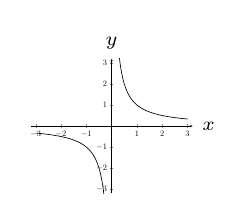
\begin{tikzpicture}[scale = .3]
\begin{axis}[axis y line=middle, axis x line=middle, xmin=-3.2, xmax=3.2, ymin=-3.2, ymax=3.2,name=myplot, ytick={-3,-2,-1,...,3}]
\addplot[{\colorone}, domain=-3:-0.2, thick, smooth]{1/x};
\addplot[{\colorone}, domain=0.2:3, thick, smooth]{1/x};
\end{axis}
\node [right] at (myplot.right of origin) {\scriptsize $x$};
\node [above] at (myplot.above origin) {\scriptsize $y$};
\end{tikzpicture}\\
$y=\sin x$ & $y=\cos x$ & $y=\dfrac{1}{x}$
\end{tabular}
\captionof{figure}{Basic Function Graphs}\label{prereq_basic_graphs}
\end{center}
\end{lxfigure}

We will often transform these functions into other functions as given in the next two figures.
\begin{lxfigure}
\begin{center}
\begin{tabular}{l c}
The function & shifts $f(x)$\\\midrule
$y=f(x)+c$ & $$c units upward\\
$y=f(x)-c$ & $c$ units downward\\
$y=f(x+c)$ & $c$ units left\\
$y=f(x-c)$ & $c$ units right\\
\end{tabular}
\captionof{figure}{Translations of Basic Functions with $c>0$}
\end{center}
\end{lxfigure}

\begin{lxfigure}
\begin{center}
\begin{tabular}{l c}
The function &  transforms $f(x)$ by\\\midrule
$y=cf(x)$ & stretching vertically by a factor of $c$\\
$y=\frac{1}{c} f(x)$ & shrinking vertically by a factor of $c$\\
$y=f(cx)$ & shrinking horizontally by a factor of $c$\\
$y=f(\frac{x}{c})$ & stretching horizontally by a factor of $c$\\
$y=-f(x)$ & reflecting about the $x$-axis\\
$y=f(-x)$ & reflecting about the $y$-axis\\
\end{tabular}
\captionof{figure}{Scaling Basic Functions with $c>1$}
\end{center}
\end{lxfigure}

%\example{ex_prereq_sketch}{Sketching with basic transformations}{Sketch the graph of the following functions using the base function and the appropriate transformations.
%\begin{enumerate}
%\begin{multicols}{2}
%\item $y=\displaystyle \frac{1}{x+3}$
%\item $y=\sqrt{x+3}+1$
%\item $y=\abs{x-4}$
%\item $y=3\cos x+2$
%\item $y=4\abs{x}+1$
%\item $y=-\frac{1}{3}(x-2)^2+3$
%\item $y=(x-3)^3$
%\item$y=\abs{\sin 2x}$
%\end{multicols}
%\end{enumerate}}{\ifthenelse{\boolean{latexml}\OR\isodd{\thepage}}{%
%% do nothing
%}{%
%\hspace{-100pt}%
%}%
%\begin{tabular}{cccc}
%\begin{tikzpicture}[scale = .5]
%\begin{axis}[axis y line=middle, axis x line=middle, xmin=-4, xmax=4, ymin=-4, ymax=4,name=myplot, ytick={0, 1,2}, xtick={0,1,2,3}]
%\addplot[{\colorone}, domain=-3:4, thick, smooth,samples=100]{1/(x+3)};
%\addplot[{\colorone}, domain=-4:-3, thick, smooth,samples=100]{1/(x+3)};
%\end{axis}
%\node [right] at (myplot.right of origin) {\scriptsize $x$};
%\node [above] at (myplot.above origin) {\scriptsize $y$};
%\end{tikzpicture}
%&
%\begin{tikzpicture}[scale = .5]
%\begin{axis}[axis y line=middle, axis x line=middle, xmin=-4, xmax=4, ymin=-4, ymax=4,name=myplot, ytick={0, 1,2}, xtick={0,1,2,3}]
%\addplot[{\colorone}, domain=-3:4, thick, smooth,samples=100]{sqrt(x+3)+1};
%\end{axis}
%\node [right] at (myplot.right of origin) {\scriptsize $x$};
%\node [above] at (myplot.above origin) {\scriptsize $y$};
%\end{tikzpicture}
%&
%\begin{tikzpicture}[scale = .5]
%\begin{axis}[axis y line=middle, axis x line=middle, xmin=-5, xmax=5, ymin=-5, ymax=5,name=myplot, ytick={0, 1,2}, xtick={0,1,2,3}]
%\addplot[{\colorone}, domain=-5:5, thick, smooth,samples=100]{abs(x-4)};
%\end{axis}
%\node [right] at (myplot.right of origin) {\scriptsize $x$};
%\node [above] at (myplot.above origin) {\scriptsize $y$};
%\end{tikzpicture}
%\end{tabular}
%}

\subsection*{Domain}

We said above that domain is the set of real numbers for which the function (rule) defines a real number and makes sense. Ask yourself, "what values can I put into the function and get a real value out?" There are generally two key expressions that will limit the domain of a function from all real numbers. We may not divide by zero and we may not have a negative number underneath an even root. The following examples illustrate how we restrict the domain when we see these expressions.

\example{prereq_domain_1}{Finding a domain}{Find the domain of the function $f(x)=\sqrt{x-4}$.}{The square root of a negative number is not defined as a real number so the domain of $f$ will be all real numbers for which $x-4\geq 0$ which is $x \geq 4$. In interval notation, this is $[4,\infty)$.}

\example{prereq_domain_2}{Finding a domain}{Find the domain of the function $g(x)= \dfrac{3}{x^2-9}$.}{We cannot divide by zero so we factor the denominator of $g$ and exclude those values where the denominator is zero.
\[g(x)=\frac3{x^2-9}=\frac3{(x-3)(x+3)}\]
We see that $x\neq 3,-3$ for $g$ to be defined, which is written in interval notation as $(-\infty,-3)\cup (-3,3)\cup (3,\infty)$.}

\example{prereq_domain_3}{Finding a domain}{Find the domain of the function $h(x)=\dfrac1{\sqrt{x^2-4}}$}{For $h$ to be defined as a real number we must have $x^2-4>0$. This is equivalent to $(x-2)(x+2)>0$. From the sign chart below, we can see that $x^2-4$ will be greater than zero on $(-\infty,-2)\cup(2,\infty)$.

\begin{center}
\begin{tikzpicture}
  \matrix[row sep=1mm,column sep=3mm,ampersand replacement=\&] {
    \&\&\& \node (tp1) {$-2$}; \&\& \node (tp2) {$2$}; \\[-1ex]
    \node(linestart) {$x$}; \&\&\&\&\&\&\& \node(lineend) {}; \\[-1ex]
    \&\node (fstart) {$x^2-4$}; \& \node {$+$}; \&\& \node {$-$}; \&\& \node {$+$}; \\
  };
  \draw [<->] (linestart.east) -- (lineend);
  \draw (fstart.south west) -- (lineend.west |- fstart.south);
  \draw (fstart.east |- lineend) -- (fstart.east|-fstart.south);
  \foreach \x in {1,2} {
    \draw (tp\x|-linestart)+(0,5pt) -- (tp\x |- fstart.south);
  };
\end{tikzpicture}\eoehere
\end{center}}

\printexercises{exercises/01_00_exercises}
